\scanpage{15}
% archive sheet number: 14

\figure{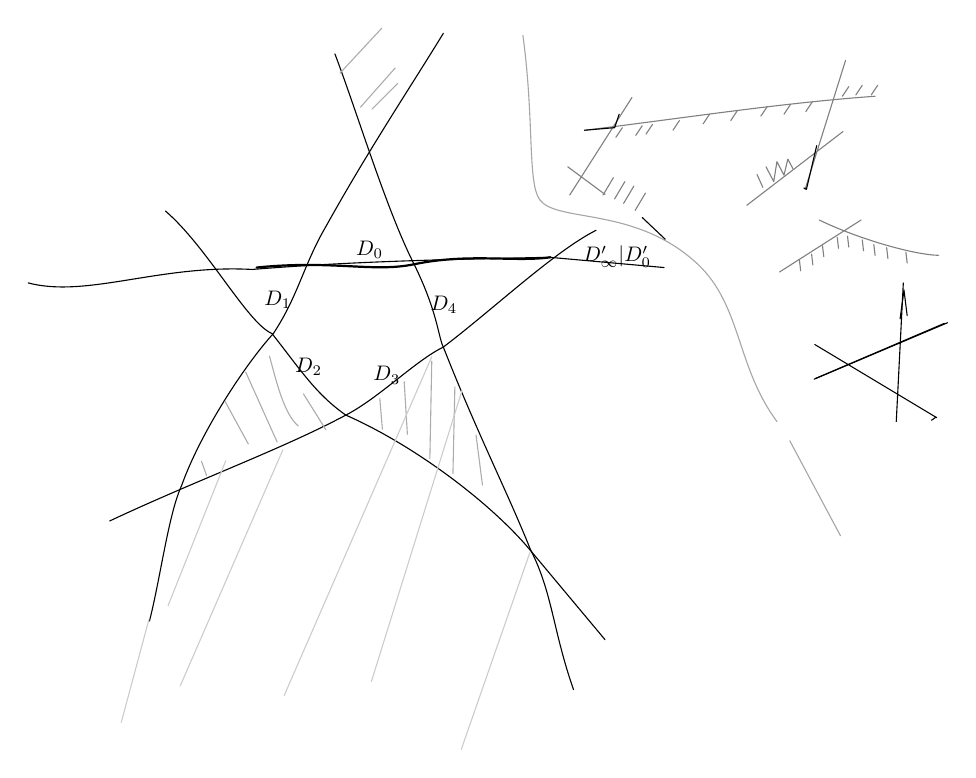
\begin{tikzpicture}[x=.00815cm,y=-.00815cm,line cap=round,line join=round,inner sep=.4pt]
% Drawing 1
\begin{scope}
\draw (212,426)..controls(303,450)and(417,397)..(561,405)..controls(733,391)and(897,389)..(1024,386)--(1203,402);
\draw[thick] (568,402)..controls(686,390)and(750,410)..(813,397)..controls(899,379)and(970,394)..(1026,386);
\draw (401,953)..controls(418,886)and(431,785)..(451,742)..controls(481,658)and(551,552)..(594,505)..controls(633,446)and(641,398)..(676,338)..controls(744,216)and(807,122)..(859,37);
\draw (426,314)..controls(492,371)and(553,488)..(592,505)..controls(637,562)and(660,599)..(707,632)..controls(814,679)and(933,769)..(994,842)--(1111,982);
\draw (339,797)..controls(480,731)and(608,685)..(709,631)..controls(760,604)and(816,547)..(859,526)..controls(938,466)and(1032,377)..(1097,344);
\draw (690,69)..controls(725,161)and(769,308)..(812,394)..controls(850,470)and(851,510)..(859,526)..controls(913,663)and(959,752)..(995,842)..controls(1029,908)and(1030,969)..(1062,1060);
\draw[gray!65] (698,99)--(763,29) (730,152)--(784,91) (748,155)--(788,115) (519,611)--(555,677) (551,565)--(600,674) (588,540)..controls(598,576)and(610,630)..(633,649) (641,599)--(676,655) (482,704)--(490,726) (760,606)--(764,654) (798,580)--(803,662) (841,548)--(838,700) (877,588)--(874,723) (910,663)--(920,741);
\draw[gray!40] (400,951)--(357,1111) (520,703)--(430,929) (609,686)--(449,1054) (841,541)--(611,1069) (888,594)--(747,1047) (994,846)--(887,1153);
\draw[gray!70] (983,40)..controls(1001,171)and(990,269)..(1009,296)..controls(1035,332)and(1152,307)..(1248,390)..controls(1325,455)and(1313,553)..(1379,642) (1399,672)--(1478,820);
\draw (1169,324)--(1205,358);
\node[scale=0.76,transform shape=false] at (744,374) {$D_0$};
\node[scale=0.76,transform shape=false] at (601,452) {$D_1$};
\node[scale=0.76,transform shape=false] at (649,557) {$D_2$};
\node[scale=0.76,transform shape=false] at (771,570) {$D_3$};
\node[scale=0.76,transform shape=false] at (860,460) {$D_4$};
\node[scale=0.76,transform shape=false] at (1130,385) {$\deleted{\unsure{D_{\infty}'|D_0'}}$};
\end{scope}
% Drawing 2
\begin{scope}
\draw[gray] (1080,188)..controls(1249,167)and(1382,146)..(1532,135) (1053,245)--(1111,288) (1056,289)--(1153,137) (1332,305)--(1482,190) (1423,280)--(1486,79);
\draw (1079,188)--(1126,184)--(1133,163) (1421,278)--(1425,280)--(1441,212);
\foreach \x/\y in {1138/184,1169/181,1185/179,1227/173,1274/163,1317/158,1364/151,1400/148,1434/144,1491/120,1512/118,1536/118}{\draw[gray] (\x,\y)--++(-10,15);}
\foreach \x/\y in {1108/289,1126/295,1140/302,1158/313}{\draw[gray] (\x,\y)--++(16,-27);}
\draw[gray] (1348,257)--(1357,277) (1362,245)--(1374,268)--(1379,237)--(1390,258)--(1396,233)--(1404,248);
\draw[gray] (1383,409)--(1510,328) (1445,328)..controls(1505,357)and(1591,382)..(1631,383);
\foreach \x/\y in {1414/390,1433/381,1450/368,1473/355,1489/353,1512/359,1530/366,1550/371,1580/378}{\draw[gray] (\x,\y)--++(2,17);}
\draw (1437,576)--(1645,488) (1438,522)--(1628,636) (1565,642)--(1576,426);
\draw (1439,575)--(1640,489) (1571,482)--(1577,437)--(1582,477) (1620,640)--(1627,635);
\end{scope}

\end{tikzpicture}}
